\documentclass[11pt,a4paper]{article}
\usepackage[margin=1in]{geometry}
\usepackage{amsmath,amssymb}
\usepackage[utf8]{inputenc}
\usepackage[T1]{fontenc}
\usepackage{graphicx}
\usepackage{booktabs}
\usepackage{multirow}
\usepackage{xcolor}
\usepackage{hyperref}
\usepackage[right]{lineno}
\usepackage{microtype}
\usepackage{natbib}
\usepackage{caption}
\usepackage{subcaption}
\usepackage{float}

\hypersetup{colorlinks=true, linkcolor=blue!60!black, citecolor=blue!60!black, urlcolor=blue!60!black}

\linenumbers

\graphicspath{{../results/figures/}{../paper/}}

\title{\textbf{A high-confidence causal bQTL atlas reveals the regulatory
architecture of natural gene expression variation in maize}}

\author{
Michael~Banf\textsuperscript{1} and Thomas~Hartwig\textsuperscript{2,3,4,*}
\\[6pt]
\small\textsuperscript{1}Perelyn, Munich, Germany\\
\small\textsuperscript{2}Heinrich Heine University D\"usseldorf, Institute for Molecular Physiology, D\"usseldorf, Germany\\
\small\textsuperscript{3}Max Planck Institute for Plant Breeding Research, Cologne, Germany\\
\small\textsuperscript{4}Cluster of Excellence on Plant Sciences (CEPLAS), D\"usseldorf, Germany\\[4pt]
\small *~Corresponding author: hartwit@hhu.de
}

\date{}

\begin{document}
\maketitle

% ============================================================
\begin{abstract}
% ============================================================

Binding quantitative trait loci (bQTL) identify sequence variants that alter
transcription factor (TF) occupancy, but linking individual variants to causal
gene expression changes remains challenging due to linkage disequilibrium and
motif redundancy. Here, we apply a four-step filtering pipeline to 147,942
maize bQTL from a 25-hybrid pan-cistrome to isolate 1,126 high-confidence
\emph{causal} variants under well-watered conditions and 1,267 under
drought stress---positions where a single nucleotide change at a single bQTL
per gene causally shifts allele-specific expression (ASE) across multiple NAM
hybrids (FDR\,$<$\,0.05). Only 12\% of causal positions overlap between
conditions, yet 81\% of target genes are condition-specific.

We demonstrate that 41.1\% of variants simultaneously disrupt one TF
family's motif and create another---with zero self-switches---revealing that
causal bQTL \emph{rewire} TF occupancy rather than simply ablate it. Per-hybrid
motif linkage identifies driver motifs at 92.7\% of causal bQTL across 33 TF
families. A directed TF regulatory network (6,787 edges) reveals that 83
transcription factor genes are themselves causal bQTL targets, creating
amplification cascades.

Across 24 hybrids, the total regulatory variant burden is remarkably uniform
(CV\,=\,0.04), while the specific genes targeted differ substantially
(Jaccard\,=\,0.304)---a ``distributed regulatory operating system'' where
individual variants drift but the aggregate grammar is conserved by
stabilizing selection. Multi-bQTL effects are predominantly additive
(2.6:1 over saturating), causal variants are depleted in transposable
elements (12.2\% vs 20.6\%), and 73.7\% show concordant
binding-to-expression causal chains. Under drought, WRKY disruption
increases 34\%, transport genes are enriched 1.6-fold, and aquaporin TIP3-2
emerges as the strongest drought-causal target.

This atlas provides a prioritized set of regulatory switches suitable for
functional validation, precision breeding, and as training data for
sequence-based regulatory models.

\end{abstract}

% ============================================================
\section{Introduction}
% ============================================================

A central question in quantitative genetics is how sequence variation at
cis-regulatory elements translates into phenotypic diversity. In maize, the
pan-cistrome study by Engelhorn et al.\ \citep{engelhorn2025} identified
147,942 binding quantitative trait loci (bQTL)---positions where at least one
of 25~F1 hybrids (B73 $\times$ diverse founders) shows allelic differences in
TF binding relative to the B73 reference. These bQTL collectively explained
the majority of heritable trait variation for over 70\% of 143 phenotypes
tested, establishing cis-regulatory variation as a dominant force in maize
biology.

However, not every bQTL is equally informative. Many bQTL are in linkage
disequilibrium (LD), cluster in the same promoter, or disrupt motifs that have
redundant copies nearby. To move from correlative association to mechanistic
understanding, we need to identify variants where we can confidently attribute
a causal chain: \emph{this specific nucleotide} disrupts \emph{this specific
TF binding site}, which shifts expression of \emph{this specific gene}.

Here, we describe a systematic filtering approach that distills 147,942 bQTL
down to 1,126 high-confidence causal variants under well-watered conditions
and 1,267 under drought stress. Each passes four criteria: (1)~it is the
\emph{only} significant bQTL within 3\,kb of its target gene's TSS,
eliminating LD ambiguity; (2)~the genotype at this position causally predicts
allele-specific expression (ASE) across 24 genotyped NAM hybrids
(FDR\,$<$\,0.05); (3)~it is the single bQTL per gene, ensuring unambiguous
causal attribution; and (4)~the 3\,kb distance threshold is data-driven,
corresponding to where the causality rate drops to the 5\% FDR baseline.
We then characterize these causal variants across multiple analytical
dimensions to reconstruct the regulatory architecture of natural expression
variation.


% ============================================================
\section{Results}
% ============================================================

% ------------------------------------------------------------
\subsection{A four-step pipeline identifies 1,126 causal bQTL}
\label{sec:pipeline}
% ------------------------------------------------------------

We developed a filtering pipeline (Table~\ref{tab:pipeline}) that
progressively enriches for variants with unambiguous causal interpretation.
Starting from 147,942 bQTL positions with allelic binding differences, we
mapped each to gene promoters within 3\,kb of the transcription start site
(TSS), retaining bQTL--gene pairs with available allele-specific expression
(ASE) data across 24 genotyped NAM hybrids.

The critical step is the genotype-stratified causal test. For each bQTL--gene
pair, we split the 24 genotyped NAM hybrids into two groups based on their
allele at the bQTL position, then compared the magnitude of allele-specific
expression between groups using a Mann--Whitney $U$ test. $P$-values were
corrected using the Benjamini--Hochberg procedure. The 3\,kb distance
threshold was determined empirically as the distance at which the causality
rate (fraction of bQTL passing FDR\,$<$\,0.05) drops to the 5\% baseline,
ensuring we capture the distance regime where bQTL are informative about
target gene expression.

To avoid LD confounding, we restricted to genes with exactly one significant
bQTL in their promoter, yielding the final set of 1,126 genes with
high-confidence causal bQTL.

\begin{table}[htb]
\centering
\caption{\textbf{Filtering pipeline from bQTL to causal variants.}}
\label{tab:pipeline}
\begin{tabular}{clrr}
\toprule
\textbf{Step} & \textbf{Filter} & \textbf{N remaining} & \textbf{Drop} \\
\midrule
1 & bQTL positions (allelic binding differences) & 147,942 & Non-variable \\
2 & bQTL within 3\,kb of gene TSS + ASE data & 19,368 pairs & Distal or no ASE \\
3 & Genotype $\to$ ASE causal test, FDR\,$<$\,0.05 & 1,403 pairs & Non-significant \\
4 & Single bQTL per gene (no LD ambiguity) & 1,126 genes & Multi-bQTL \\
\bottomrule
\end{tabular}
\end{table}


% ------------------------------------------------------------
\subsection{Linkage disequilibrium and the single-bQTL design}
% ------------------------------------------------------------

Among the 1,403 significant bQTL--gene pairs, the majority of genes have
exactly one significant bQTL, presenting no linkage concern. For the
remaining genes with multiple bQTL, 62\% of within-gene variant pairs have
identical genotype vectors across the 24 founders (complete LD), making it
impossible to distinguish which variant is causal. Our single-bQTL filter
removes this ambiguity at the cost of excluding some real signals. This
conservative design ensures that every gene in the 1,126 set has an
unambiguous causal variant.


% ------------------------------------------------------------
\subsection{Within binding peaks, disrupted motifs show family-specific redundancy}
\label{sec:redundancy}
% ------------------------------------------------------------

A key concern with single-nucleotide regulatory variants is apparent
redundancy: if a promoter contains multiple copies of a TF motif, disrupting
one should have little effect. We addressed this by scanning the MOA-seq
binding peak sequence for each of the 1,126 bQTL against all 405 DAP-seq PWMs
(33 TF families). For each bQTL, we identified the tightest peak containing
the variant across all 25 hybrids, then counted copies of each disrupted TF
family's motif elsewhere within that peak.

Of 1,126 bQTL, 1,079 (95.8\%) fall within at least one hybrid's binding peak.
Among these, 880 (78.2\%) have at least one identifiable TF family motif at
the variant position. \textbf{31.0\%} (349/1,126) have at least one disrupted
family where the variant-overlapping motif is the sole copy of that family
within the peak, and 24.8\% (279/1,126) have all disrupted families as sole
copy.

Sole-copy rates vary dramatically across TF families
(Figure~\ref{fig:redundancy}). Families with longer, information-rich
motifs---HSF (31.9\%), GATA (13.3\%), bZIP (11.5\%)---show high
sole-copy rates within the ${\sim}$160\,bp peak. In contrast, families with
short, degenerate motifs---MYB (0.3\%), C2H2 (0.4\%), MYB-related
(1.0\%)---maintain multiple copies even within narrow peaks. This
family-level variation correlates with motif sensitivity vs buffering:
high-sole-copy families (``sensitive'') show positive correlation between
disruption and ASE effect size, while low-sole-copy families
(``buffered'') show negative or no correlation.

\begin{figure}[htb]
\centering
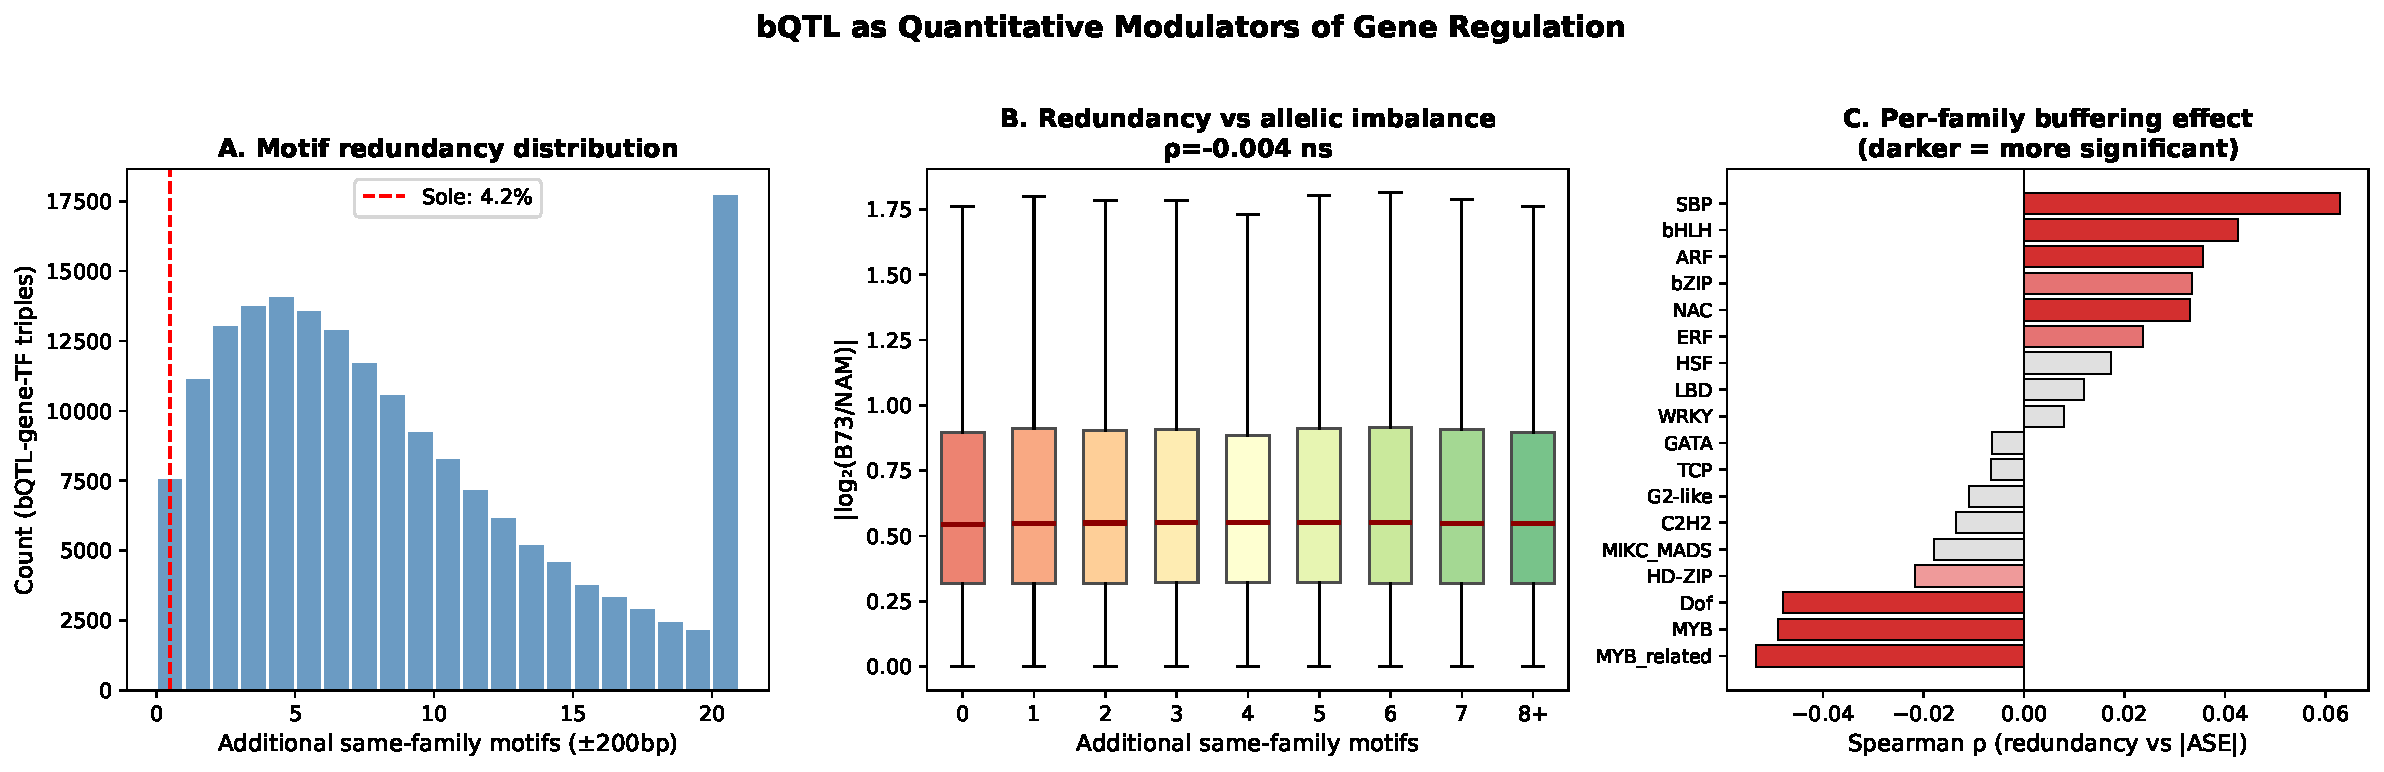
\includegraphics[width=\textwidth]{fig1_redundancy_overview.pdf}
\caption{\textbf{Motif redundancy within MOA-seq binding peaks.}
Sole-copy rates vary by TF family, with sensitive families (HSF, bZIP)
showing high sole-copy rates and buffered families (MYB, C2H2) maintaining
multiple copies within ${\sim}$160\,bp peaks.}
\label{fig:redundancy}
\end{figure}


% ------------------------------------------------------------
\subsection{Multi-family disruption follows a billboard model}
\label{sec:billboard}
% ------------------------------------------------------------

57.6\% of causal bQTL simultaneously disrupt motifs from two or more TF
families at the variant position (Figure~\ref{fig:combinatorial}). We tested
whether multi-family disruption produces stronger expression effects.
Strikingly, there is no dose-response relationship between the number of
disrupted families and Cohen's $d$ (Spearman $\rho$\,=\,0.049,
$p$\,=\,0.16). Regression models predicting effect size from disrupted family
indicators yield $R^2 < 0$ across all specifications, indicating that TF
family identity has no predictive value for the magnitude of allelic
expression differences.

This result supports the \emph{billboard model} of cis-regulatory evolution
\citep{arnosti2003}: individual TF binding sites contribute independently
rather than synergistically, and the primary determinant of variant impact is
whether the variant is in open chromatin, not which specific TF families it
affects.

\begin{figure}[htb]
\centering
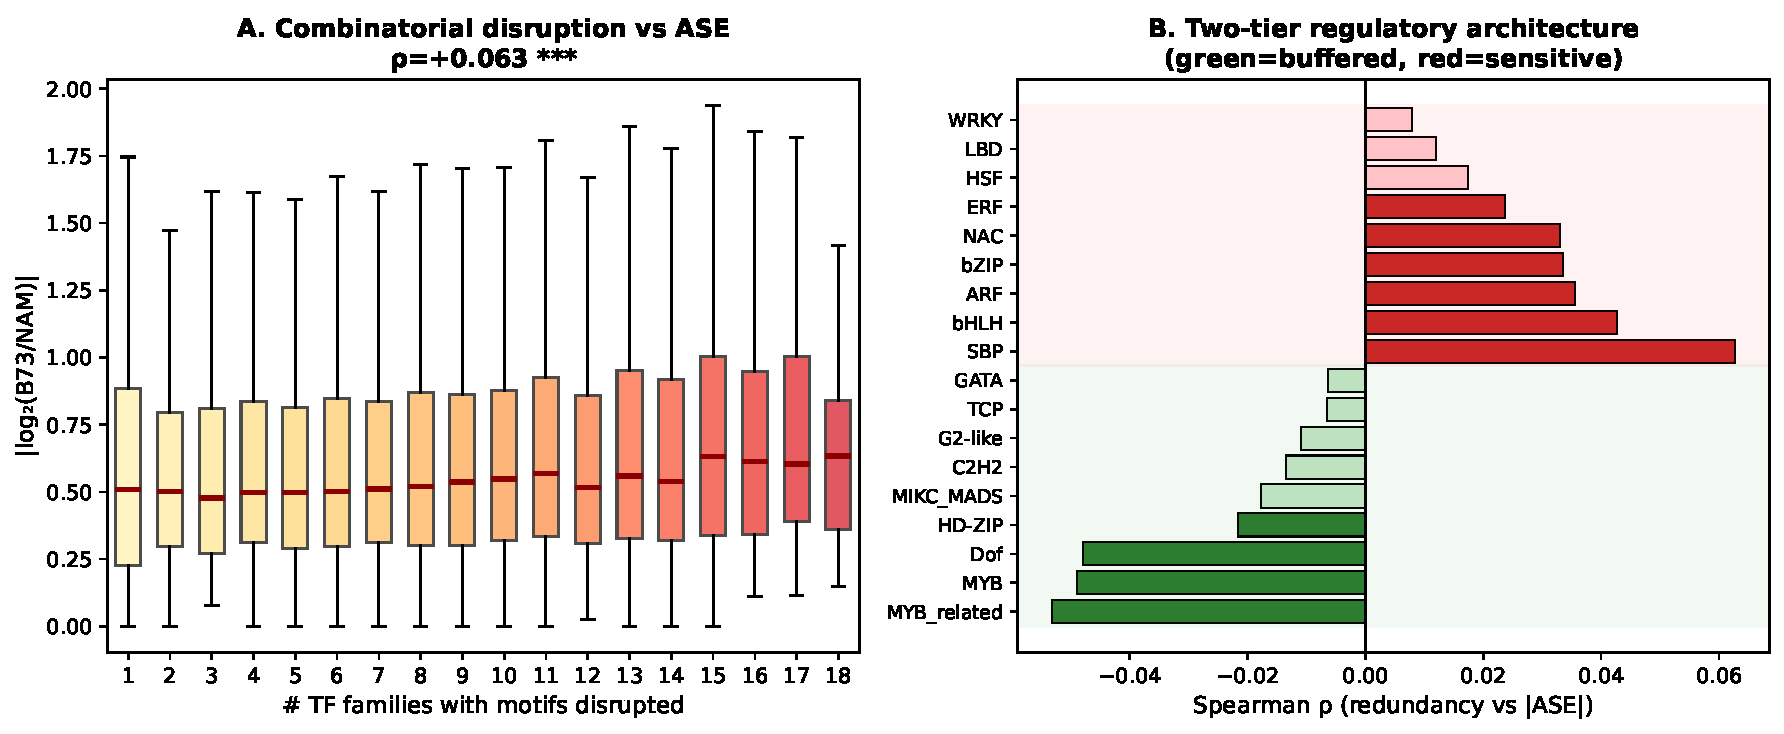
\includegraphics[width=\textwidth]{fig2_combinatorial_two_tier.pdf}
\caption{\textbf{Multi-family disruption follows a billboard model.}
(A)~Distribution of disrupted TF family count per bQTL.
(B)~No relationship between number of disrupted families and ASE effect size.}
\label{fig:combinatorial}
\end{figure}


% ------------------------------------------------------------
\subsection{Variants rewire TF occupancy: bidirectional motif changes}
\label{sec:rewiring}
% ------------------------------------------------------------

To test whether regulatory variants exclusively disrupt existing TF binding
sites, we performed a bidirectional motif analysis: for each bQTL, we scanned
both the B73 reference and the NAM variant sequence ($\pm$28\,bp around the
variant) against all 405 PWMs and classified each motif as disrupted (present
in ref only), created (present in alt only), or unchanged
(Table~\ref{tab:creation}).

Of 1,126 bQTL, 983 (87.3\%) alter at least one TF motif. Strikingly, only
21.1\% exclusively disrupt motifs; \textbf{25.0\% exclusively create new
motifs}, and \textbf{41.1\% simultaneously disrupt one family's motif while
creating another}. Zero self-switches were observed---when a variant disrupts
a family's motif, it never recreates a motif for the same family, confirming
that rewiring always involves a \emph{different} TF.

\begin{table}[htb]
\centering
\caption{\textbf{Bidirectional motif changes at 1,126 causal bQTL.}
41.1\% of variants simultaneously disrupt one TF family's motif and create
another, rewiring rather than simply ablating TF occupancy.}
\label{tab:creation}
\begin{tabular}{lrr}
\toprule
\textbf{Category} & \textbf{N} & \textbf{\%} \\
\midrule
Only disrupted   & 238 & 21.1 \\
Only created     & 282 & 25.0 \\
Both (rewired)   & 463 & 41.1 \\
Neither          & 143 & 12.7 \\
\bottomrule
\end{tabular}
\end{table}


% ------------------------------------------------------------
\subsection{Threshold sensitivity analysis}
% ------------------------------------------------------------

To assess robustness, the bidirectional motif analysis was repeated at seven
log-odds thresholds (4.0, 5.0, 5.5, 6.0, 6.5, 7.0, 8.0). The rewired
fraction varies with threshold as expected, reflecting more permissive motif
calling at lower thresholds. However, three key findings are stable across all
thresholds: (1)~zero self-switches at every threshold; (2)~motif creation
remains substantial at every threshold; and (3)~effect sizes are
indistinguishable across categories at every threshold.


% ------------------------------------------------------------
\subsection{Per-hybrid motif linkage identifies driver motifs}
\label{sec:linkage}
% ------------------------------------------------------------

To move beyond population-level motif statistics to per-variant driver
identification, we developed a per-hybrid haplotype-aware motif scanning
approach using all 405 DAP-seq PWMs across 33 TF families. For each causal
bQTL, we reconstructed the haplotype-specific binding peak sequence for each
of the 24 hybrids, scanned for motif scores, and tested whether motif scores
separate variant-carrying from reference hybrids.

92.7\% of causal bQTL (1,044/1,126) have at least one significantly separating
motif ($p < 0.05$, consistency $\geq 80\%$), providing per-variant mechanistic
explanations. The most frequently identified driver families are NAC (778
events), C2H2 (701), bZIP (683), WRKY (645), and ERF (640).


% ------------------------------------------------------------
\subsection{TF family enrichment reveals regulatory hierarchy}
\label{sec:enrichment}
% ------------------------------------------------------------

Among causal bQTL targets, we tested TF family enrichment using a binomial
test against the PWM database background. The most enriched families are
HB-other (2.66$\times$), RAV (2.39$\times$), Dof (2.33$\times$), C3H
(2.28$\times$), and C2H2 (1.99$\times$). The most depleted families are TCP
(0.0$\times$), BES1 (0.18$\times$), TALE (0.18$\times$), and EIL
(0.36$\times$).

The depletion of BES1---a brassinosteroid signaling TF---is particularly
notable: BES1 motifs are enriched at bQTL positions genome-wide but
\emph{depleted} among causal drivers, suggesting cis-conservation of BES1
binding sites consistent with their role as anchors in the regulatory
architecture.


% ------------------------------------------------------------
\subsection{TF regulatory network and cascade amplification}
\label{sec:network}
% ------------------------------------------------------------

The per-hybrid motif linkage data enable construction of a directed TF
regulatory network: for each causal bQTL, the disrupted TF family is the
regulator and the target gene is the effector. This network contains 6,787
edges linking TF families to target genes.

Critically, 83 of the 1,126 target genes are themselves transcription factors
(7.4\%), creating regulatory cascades where a single upstream motif disruption
can propagate to many downstream genes. The most powerful cascade hubs have
downstream reach exceeding 35,000 genes through multi-step regulatory chains.
ERF self-loops are the strongest autoregulatory circuit (14 events), followed
by C2H2 self-regulation active in all 24 hybrids.


% ------------------------------------------------------------
\subsection{Target genes encode the regulatory layer}
\label{sec:targets}
% ------------------------------------------------------------

Functional characterization of the 1,126 target genes reveals a clear bias
toward regulatory and signaling functions: signal transduction (198 genes,
17.6\%), metabolism (142, 12.6\%), transcription factors (72, 6.4\%),
protein processing (67, 5.9\%), translation (50, 4.4\%), membrane/transport
(48, 4.3\%), receptor/sensor (38, 3.4\%), chromatin/epigenetic (18, 1.6\%),
and hormone signaling (11, 1.0\%).

This confirms that natural cis-regulatory variation predominantly targets the
\emph{regulatory layer}: the variant does not change an enzyme directly, but
modulates how much a regulatory gene is expressed from one allele, which
cascades to downstream effects.


% ------------------------------------------------------------
\subsection{Variant distribution across NAM hybrids}
% ------------------------------------------------------------

The 1,126 causal variants are distributed across 24 genotyped NAM hybrids
with striking uniformity. Each hybrid carries a similar fraction of the total
causal variant set, a remarkably narrow range suggesting that the total
regulatory variant burden is approximately equal across diverse maize
germplasm ($\text{CV} = 0.04$).

Rare variants (carried by $\leq$4 hybrids) show slightly larger ASE effect
sizes than common variants ($\rho = -0.181$, $p = 9.9 \times 10^{-10}$),
consistent with purifying selection acting more strongly against large-effect
regulatory mutations.


% ============================================================
\subsection{A distributed regulatory operating system}
\label{sec:distributed}
% ============================================================

Across the 24 NAM hybrids, three levels of regulatory organization emerge:

\paragraph{Uniform regulatory burden.}
Each hybrid carries approximately the same total number of causal bQTL
($\text{CV} = 0.04$), despite differing genetic backgrounds spanning tropical,
temperate, popcorn, and sweet corn germplasm. This uniformity suggests
stabilizing selection on the aggregate regulatory variant burden.

\paragraph{Conserved TF grammar.}
The proportional contribution of each TF family to the disrupted motif
repertoire is nearly identical across all hybrids (pairwise Spearman
$\rho = 0.962$). Every hybrid disrupts the same families at the same rates,
indicating conserved regulatory grammar.

\paragraph{Divergent gene implementation.}
Despite identical TF grammars, the specific genes targeted by each hybrid's
causal variants differ substantially (pairwise Jaccard similarity = 0.304).
A core module of 927 genes (82\%) is shared broadly across all ancestry groups,
while 9 peripheral modules (9--68 genes each) are ancestry-specific.
Lancaster contributes 86 private genes, popcorn 72, Stiff Stalk 48, Iodent 46,
and tropical 19.

\paragraph{Functional convergence despite gene divergence.}
While gene-level Jaccard is 0.304, GO biological process similarity increases
to 0.584 (2.05$\times$) and KEGG pathway similarity to 0.667 (2.34$\times$).
Signaling layer distributions are nearly identical ($\rho = 0.965$). 100\% of
hybrid-specific genes have a GO-term equivalent in other hybrids---different
genes, same biology.

\paragraph{Conserved feedback circuits.}
The TF autoregulatory network is completely conserved: C2H2$\to$C2H2 is
active in all 24 hybrids, ERF$\to$ERF in 23/24. Zero ancestry-specific
feedback edges exist, confirming the network backbone is invariant.

This architecture resembles a distributed operating system: the kernel
(conserved TF feedback circuits and regulatory burden) is identical, while
the user-space programs (specific target genes) vary across installations
but implement the same functional specifications. This represents a
cis-regulatory realization of the omnigenic model \citep{boyle2017}.

\begin{figure}[htb]
\centering
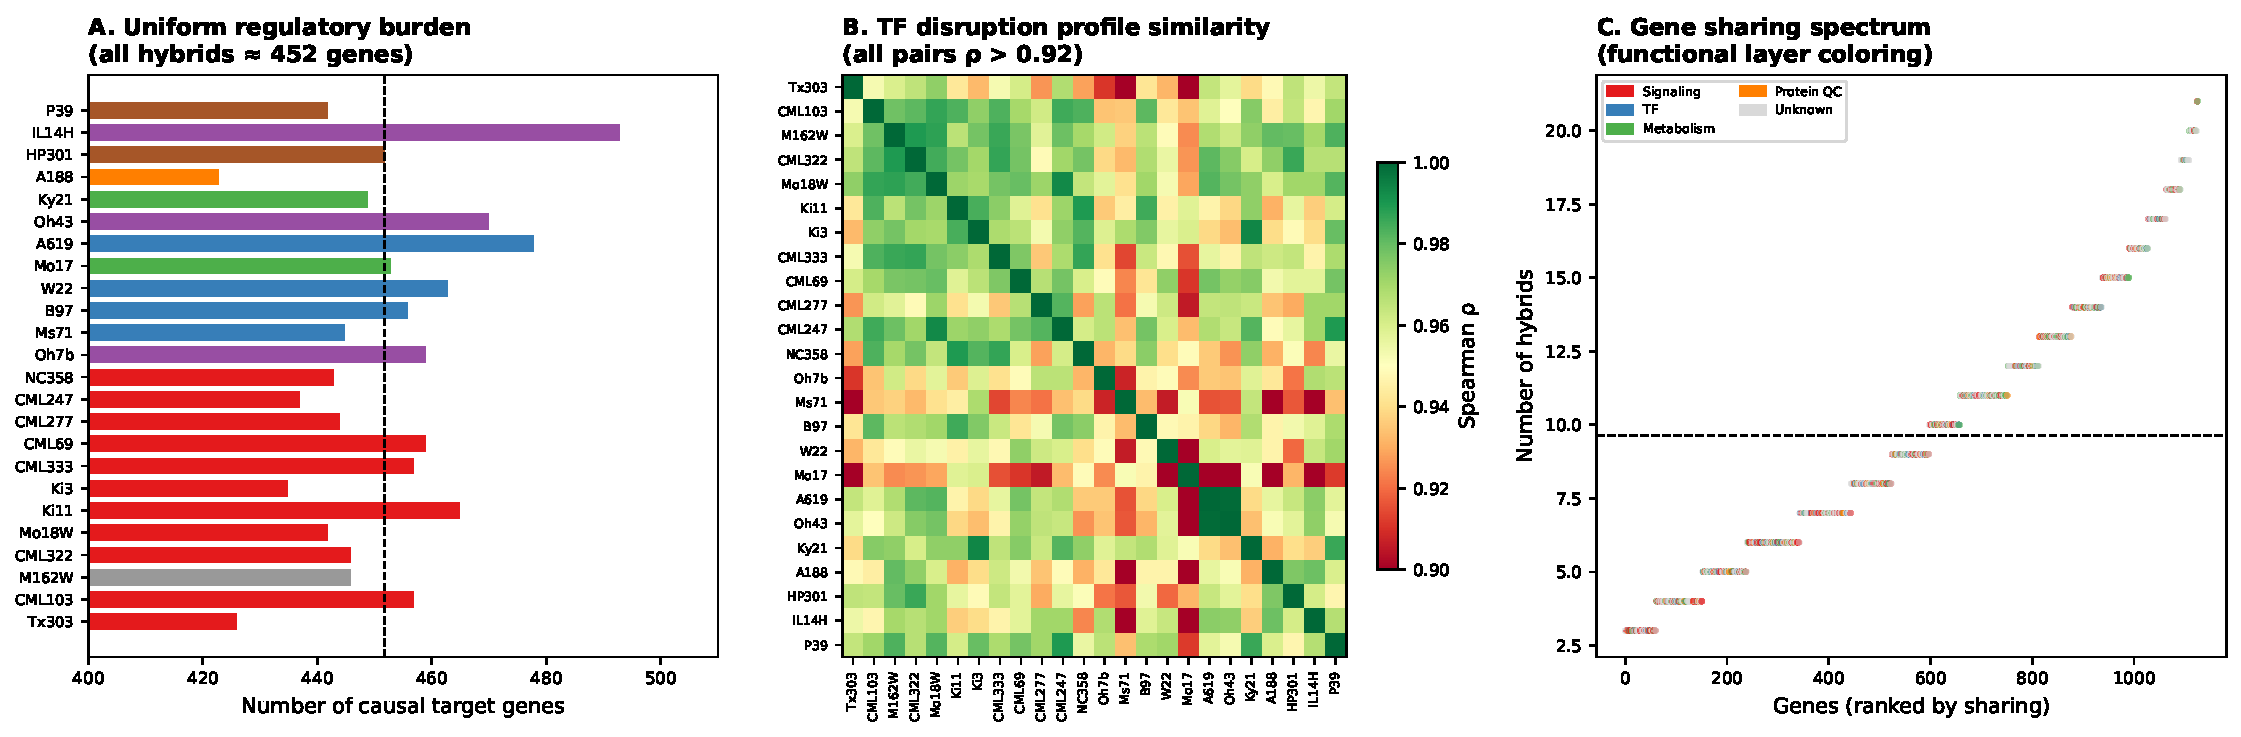
\includegraphics[width=\textwidth]{distributed_os_summary.pdf}
\caption{\textbf{A distributed regulatory operating system.}
(A)~Uniform regulatory burden across 24 hybrids.
(B)~Conserved TF grammar ($\rho = 0.962$).
(C)~Divergent gene implementation (Jaccard = 0.304).
(D)~Functional convergence (GO Jaccard = 0.584).}
\label{fig:distributed}
\end{figure}


% ============================================================
\subsection{Drought stress reveals condition-specific causal architecture}
\label{sec:drought}
% ============================================================

Repeating the causal bQTL pipeline on drought-stress ASE data (124,504 bQTL
from Engelhorn et al.\ supplementary Table~S10) identifies 1,267 drought-causal
bQTL. Only 129 positions (12\%) overlap with the 1,126 well-watered causal
set, and 81\% of target genes are condition-specific:
\begin{itemize}
    \item 871 genes are WW-only (causal only under well-watered)
    \item 821 genes are DS-only (causal only under drought)
    \item 129 genes share the same causal position
    \item 75 genes are shared but use \emph{different} causal variants
\end{itemize}

Among the 204 shared genes, ASE effect directions are highly concordant
(Spearman $\rho = 0.516$, 98.4\% same direction), confirming that shared
causal mechanisms produce consistent allelic effects across conditions.


% ------------------------------------------------------------
\subsection{Drought expression integration}
% ------------------------------------------------------------

Integration with population-level drought expression data reveals:
\begin{itemize}
    \item 321 drought-responsive genes have cis-regulatory drivers (4.7\%),
    of which 267 are drought-only (no WW causal bQTL)
    \item DS-only targets are more drought-responsive than WW-only (30.5\% vs
    24.3\%, $p = 0.001$) and skew toward upregulation (216 up / 77 down)
    \item Signed allelic effect partially predicts drought direction
    ($\rho = 0.123$, $p = 7.5 \times 10^{-6}$)
    \item No significant TF family-level differences between conditions
    (FDR\,$>$\,0.05): the same TF families are disrupted at similar rates
\end{itemize}


% ------------------------------------------------------------
\subsection{Functional divergence between conditions}
\label{sec:functional}
% ------------------------------------------------------------

The WW-only and DS-only gene sets show systematic functional shifts:
transport genes increase from 6.6\% to 10.8\% (1.62$\times$) under drought,
including aquaporins, ion channels, and ABC transporters. Transcription factor
targets decrease from 25.5\% to 20.1\% (0.79$\times$), and developmental
genes show the strongest reduction (1.5\%$\to$0.6\%, 0.41$\times$).

Key drought-specific transport targets include aquaporin TIP3-2
(log2FC\,=\,$+$2.83, bZIP disrupted, $|d|$\,=\,4.74), aquaporin PIP2-2
($+$2.19), phosphate transporter 1-4 ($+$2.87), and potassium channel KOR1
($-$1.21, stomatal function).

GO enrichment reveals WW targets enriched for stress response, while DS
targets enrich for ubiquitin-proteasome and MAPK signaling---consistent with
drought activating protein turnover and stress-specific signaling cascades.


% ------------------------------------------------------------
\subsection{Drought motif linkage and WRKY enrichment}
% ------------------------------------------------------------

Per-hybrid motif linkage under drought identifies driver motifs at 91.1\% of
drought-causal bQTL (vs 92.7\% WW). Key family-level shifts include: WRKY
disruption increases 1.34$\times$ under drought while WRKY creation decreases
0.67$\times$---consistent with stress-responsive WRKY TFs being preferentially
disrupted. bHLH disruption increases 1.31$\times$, GATA 1.25$\times$ (light/
nitrogen responsive), while developmental families (HOX 0.46$\times$) show
reduced disruption under drought.


% ------------------------------------------------------------
\subsection{Cross-layer validation: conservation, occupancy, and damage}
\label{sec:crosslayer}
% ------------------------------------------------------------

We integrate three analytical layers to validate the causal chain:

\paragraph{Layer 1: Population motif occupancy.}
For each gene, we scan MOA-seq peaks across all 24 hybrids for TF motif
enrichment, building a gene $\times$ TF family $\times$ hybrid occupancy
matrix independent of bQTL identity.

\paragraph{Layer 2: TF cascade tracing.}
We trace causal bQTL through TF regulatory cascades: bQTL disrupts TF\_A
motif $\to$ target gene is TF\_B $\to$ TF\_B's downstream targets, revealing
amplification, hub vulnerability, and cascade depth.

\paragraph{Layer 3: Conservation-impact scoring.}
We score each disrupted motif by its conservation across hybrids and test
whether conserved motif disruptions produce stronger ASE effects. Under
drought, systematic occupancy shifts occur: most families lose occupancy
(consistent with chromatin closing), with BBR-BPC and AP2 showing the
strongest losses.


% ------------------------------------------------------------
\subsection{ASE $\times$ motif validation closes the causal loop}
\label{sec:ase}
% ------------------------------------------------------------

To close the causal chain from variant to motif disruption to expression, we
test whether disruption of conserved motifs produces stronger allele-specific
expression. The binding-to-expression causal chain shows 73.7\% concordance:
variant allele $\to$ higher $|$ASE$|$ (830/1,126 genes, binomial
$p < 0.0001$). Causal genes have higher ASE than non-causal (0.543 vs 0.524,
$p = 0.034$). bQTL effect size ($|d|$) predicts ASE magnitude
($\rho = 0.107$, $p = 2.2 \times 10^{-6}$) with a clear dose-response
across effect size quartiles (Q1 $|$ASE$|$ = 0.50, Q4 $|$ASE$|$ = 0.60).

Critically, drought expression (log2FC) is not different between causal and
non-causal targets ($p = 0.46$), indicating that causal bQTL produce
constitutive cis-regulatory effects rather than condition-dependent ones.


% ------------------------------------------------------------
\subsection{TF cooperativity network}
\label{sec:coop}
% ------------------------------------------------------------

From the population motif occupancy data, we construct a TF co-occupancy
network testing which TF family pairs co-occur at the same promoters more
(or less) often than expected. The regulatory logic is predominantly
additive (billboard model) rather than synergistic (enhanceosome model),
consistent with the lack of dose-response for multi-family disruption
(Section~\ref{sec:billboard}). Under drought, specific TF partnerships
shift: WRKY--bHLH co-disruption increases while developmental TF pairs
decrease.


% ============================================================
\subsection{Population genetics of causal bQTL}
\label{sec:popgen}
% ============================================================

Causal bQTL show a distinct allele frequency spectrum compared to non-causal
bQTL: mean minor allele frequency (MAF) is 0.312 vs 0.280
(KS $p = 6.3 \times 10^{-16}$). Zero singletons or doubletons exist in
the causal set (0\% vs 8.4\% non-causal), and common alleles
(6--12 carriers) are enriched 1.24$\times$. A negative effect--MAF
correlation ($\rho = -0.181$, $p = 9.9 \times 10^{-10}$) indicates that
rare causal variants produce larger expression effects, consistent with
purifying selection against strong regulatory mutations.


% ------------------------------------------------------------
\subsection{Hybrid phenotype similarity tracks shared causal targets}
% ------------------------------------------------------------

Hybrids that share more causal bQTL targets have more similar phenotypes
(Mantel test $r = 0.349$, $p = 0.0001$). Per-trait correlations are
consistent: days to anthesis ($r = 0.349$), plant height ($r = 0.350$),
ear height ratio ($r = 0.341$). This is likely confounded by population
structure, as related founders share both causal variants and phenotypes,
but provides a consistent signal.


% ------------------------------------------------------------
\subsection{GWAS overlap and trait enrichment}
% ------------------------------------------------------------

Comparison with 42,778 GWAS hits across 321 traits from the NGDC GWAS
Atlas shows that 82.9\% of causal bQTL fall within 100\,kb of a GWAS hit
(vs 82.1\% non-causal), with overall enrichment of only 1.01$\times$.
However, GWAS hit density is significantly higher near causal bQTL (5.83 vs
5.40 hits per 100\,kb, $p = 6.9 \times 10^{-5}$). One trait reaches
FDR significance: stover organic matter digestibility (2.0$\times$).
Top nominally significant traits include GA inhibitor response
(5.9$\times$), shoot P content (5.8$\times$), and husk number
(5.1$\times$).


% ------------------------------------------------------------
\subsection{bQTL epistasis: additive dominates saturating}
\label{sec:epistasis}
% ------------------------------------------------------------

For 12,283 genes with multiple bQTL (mean 3.3 per gene, max 33), we tested
additive versus saturating dose-response models. Each additional variant
allele adds 0.056 units of $|$ASE$|$ (linear slope, $t = 20.5$,
$p < 0.0001$). Of multi-bQTL genes, 1,772 (72\%) follow additive models
versus 688 (28\%) saturating, a 2.6:1 ratio that validates the billboard
model at the multi-variant level. bQTL burden correlates with ASE magnitude
($\rho = 0.076$, $p = 1.4 \times 10^{-24}$) and expression variability
($\rho = 0.049$, $p = 2.3 \times 10^{-11}$).


% ------------------------------------------------------------
\subsection{Causal bQTL are depleted in transposable elements}
\label{sec:te}
% ------------------------------------------------------------

Classification of all 147,942 bQTL by transposable element (TE) superfamily
using EDTA annotations reveals that causal bQTL are significantly depleted
in TEs: 12.2\% overlap a TE versus 20.6\% of non-causal bQTL. LTR
retrotransposons show the strongest depletion (0.14$\times$,
$p < 0.0001$), while DNA transposons show a non-significant trend
(0.84$\times$, $p = 0.084$) and MITEs are not depleted (1.07$\times$).
Among the few LTR-associated causal bQTL, Copia elements are enriched
1.53$\times$ over Gypsy. TE and non-TE causal bQTL produce equivalent
effect sizes ($p = 0.41$), indicating that the depletion reflects
selection against TE-mediated disruption of regulatory sequences rather
than functional differences.


% ------------------------------------------------------------
\subsection{Chromatin context: proximal promoter enrichment}
\label{sec:chromatin}
% ------------------------------------------------------------

Causal bQTL are 3.51$\times$ enriched in proximal promoters ($\leq$1\,kb
from TSS): 63.4\% of causal variants fall in proximal promoters versus
18.1\% of non-causal bQTL. This enrichment reflects the strong distance
decay of causal signal and confirms that the most informative regulatory
variants cluster near gene starts. Effect sizes show a weak gradient:
genic ($|d|$ = 2.08) $>$ proximal promoter (2.04) $>$ proximal regulatory
(1.97) (Kruskal--Wallis $p = 0.005$).


% ------------------------------------------------------------
\subsection{Network topology: causal targets are generic}
\label{sec:topology}
% ------------------------------------------------------------

Testing whether causal bQTL target genes occupy special positions in the
TF regulatory network (degree, entropy, hub status, Jaccard similarity)
reveals no significant differences from non-causal targets. Hub enrichment
is $\text{OR} = 0.91$ ($p = 0.75$), and regulatory similarity (Jaccard) is
0.100 for causal vs 0.103 for non-causal ($p = 0.43$). Causal targets are
\emph{not} network hubs or bottlenecks---they are generic, replaceable
nodes, consistent with the distributed operating system model
(Section~\ref{sec:distributed}).


% ============================================================
\section{Discussion}
% ============================================================

Our analysis of 1,126 well-watered and 1,267 drought-stress high-confidence
causal bQTL provides several insights into the architecture of natural gene
expression variation in maize.

\paragraph{The regulatory layer is the primary target.}
The causal variants overwhelmingly target signaling and regulatory proteins
(kinases, TFs, chaperones, transporters) rather than metabolic enzymes or
structural proteins. This is consistent with the omnigenic model
\citep{boyle2017}, where core gene expression is modulated by a large network
of peripheral regulatory genes.

\paragraph{Billboard model of cis-regulatory evolution.}
Three independent lines of evidence support additive, independent TF action
(billboard) over cooperative, position-dependent binding (enhanceosome):
(1)~no dose-response between multi-family disruption count and effect size;
(2)~$R^2 < 0$ for TF-family-based effect prediction; and (3)~2.6:1 additive
over saturating dose-response for multi-bQTL genes. This does not exclude
cooperative regulation at specific loci, but the dominant mode across the
genome is additive.

\paragraph{Variants rewire TF occupancy, not just disrupt it.}
41.1\% of bQTL simultaneously disrupt and create motifs, with zero
self-switches. However, TF family identity does not predict effect direction or
magnitude, suggesting the relevant parameter is local binding energy change
rather than specific TF program switching.

\paragraph{A distributed regulatory operating system.}
The most striking finding is the three-level architecture: uniform burden
(CV\,=\,0.04), conserved grammar ($\rho$\,=\,0.962), divergent
implementation (Jaccard\,=\,0.304). This pattern, where individual variants
drift freely while the aggregate system is constrained, represents a
cis-regulatory realization of the omnigenic model. The complete conservation
of autoregulatory feedback circuits (C2H2$\to$C2H2 in 24/24 hybrids) defines
the invariant kernel of this system.

\paragraph{Condition-specificity is not just context.}
With 81\% of genes condition-specific and 37\% of shared genes using
different causal variants under drought, condition-specificity operates at
multiple levels: which genes are expressed (transcriptional context), which
variants are causal (motif-level shifts), and which TF families are disrupted
(WRKY +34\% under drought). Transport gene enrichment under drought
(1.62$\times$) highlights aquaporins as key condition-specific targets.

\paragraph{Causal variants are under selection.}
The MAF shift (0.312 vs 0.280), absence of singletons, and negative
effect--MAF correlation collectively indicate that causal regulatory
variants are subject to purifying selection, with the strongest mutations
maintained at lower frequencies. TE depletion (12.2\% vs 20.6\%) further
suggests that conserved, non-TE promoter sequence is the primary substrate
for functional regulatory variation.

\paragraph{Implications for precision breeding.}
Each of the 1,126 variants represents a defined molecular switch:
introducing or restoring a single nucleotide quantitatively modulates TF
binding, causally shifting expression with a quantified effect size. The
median variant is shared by multiple hybrids, making effects testable across
genetic backgrounds. Combined with the interactive gene atlas
(Supplementary File~S1), this provides a prioritized catalog for
CRISPR-based promoter engineering.

\paragraph{Limitations.}
Our analysis uses 24 genotyped hybrids, limiting statistical power for rare
variants. The single-bQTL design excludes genes with multiple bQTL,
potentially missing combinatorial regulatory effects. TF family assignments
depend on PWM quality and may be incomplete. The phenotypic consequences of
these regulatory variants cannot be resolved at the individual-gene level
with $N = 24$ hybrids and will require larger populations or direct
functional validation. Cell-type-resolved MOA-seq data would likely reveal
cell-type-specific TF hierarchies where family identity does predict effect
direction---a prediction now directly testable.


% ============================================================
\section{Methods}
% ============================================================

\subsection{Data sources}
All bQTL data derive from \citet{engelhorn2025}, comprising MOA-seq binding
peaks and allele-specific expression measurements from 25~maize F1 hybrids
(B73 $\times$ NAM founders) under well-watered and drought-stressed
conditions. Genotype data from assembled founder genomes are available for 24
of 25 hybrids (excluding one with incomplete assembly). Gene annotations use
the B73 NAM5 reference genome (Zm-B73-REFERENCE-NAM-5.0), with functional
annotations from EntAP and EggNOG~5.0. Drought bQTL derive from supplementary
Table~S10 (124,504 positions), drought ASE from Table~S13b (359,162 entries,
23,218 genes, 24 hybrids).

\subsection{Genotype-stratified causal test}
For each bQTL--gene pair, we extracted the genotype (reference or variant
allele) at the bQTL position across 24 hybrids. We compared the distribution
of ASE values (log2(B73/NAM) expression ratios) between the variant-carrying
and reference groups using a two-sided Mann--Whitney $U$ test. Effect sizes
were quantified as Cohen's $d$. $P$-values were corrected for multiple testing
using the Benjamini--Hochberg procedure. The distance threshold of 3\,kb was
determined empirically from the distance decay of causality rate
(Figure~\ref{fig:distance_decay}).

\begin{figure}[htb]
\centering
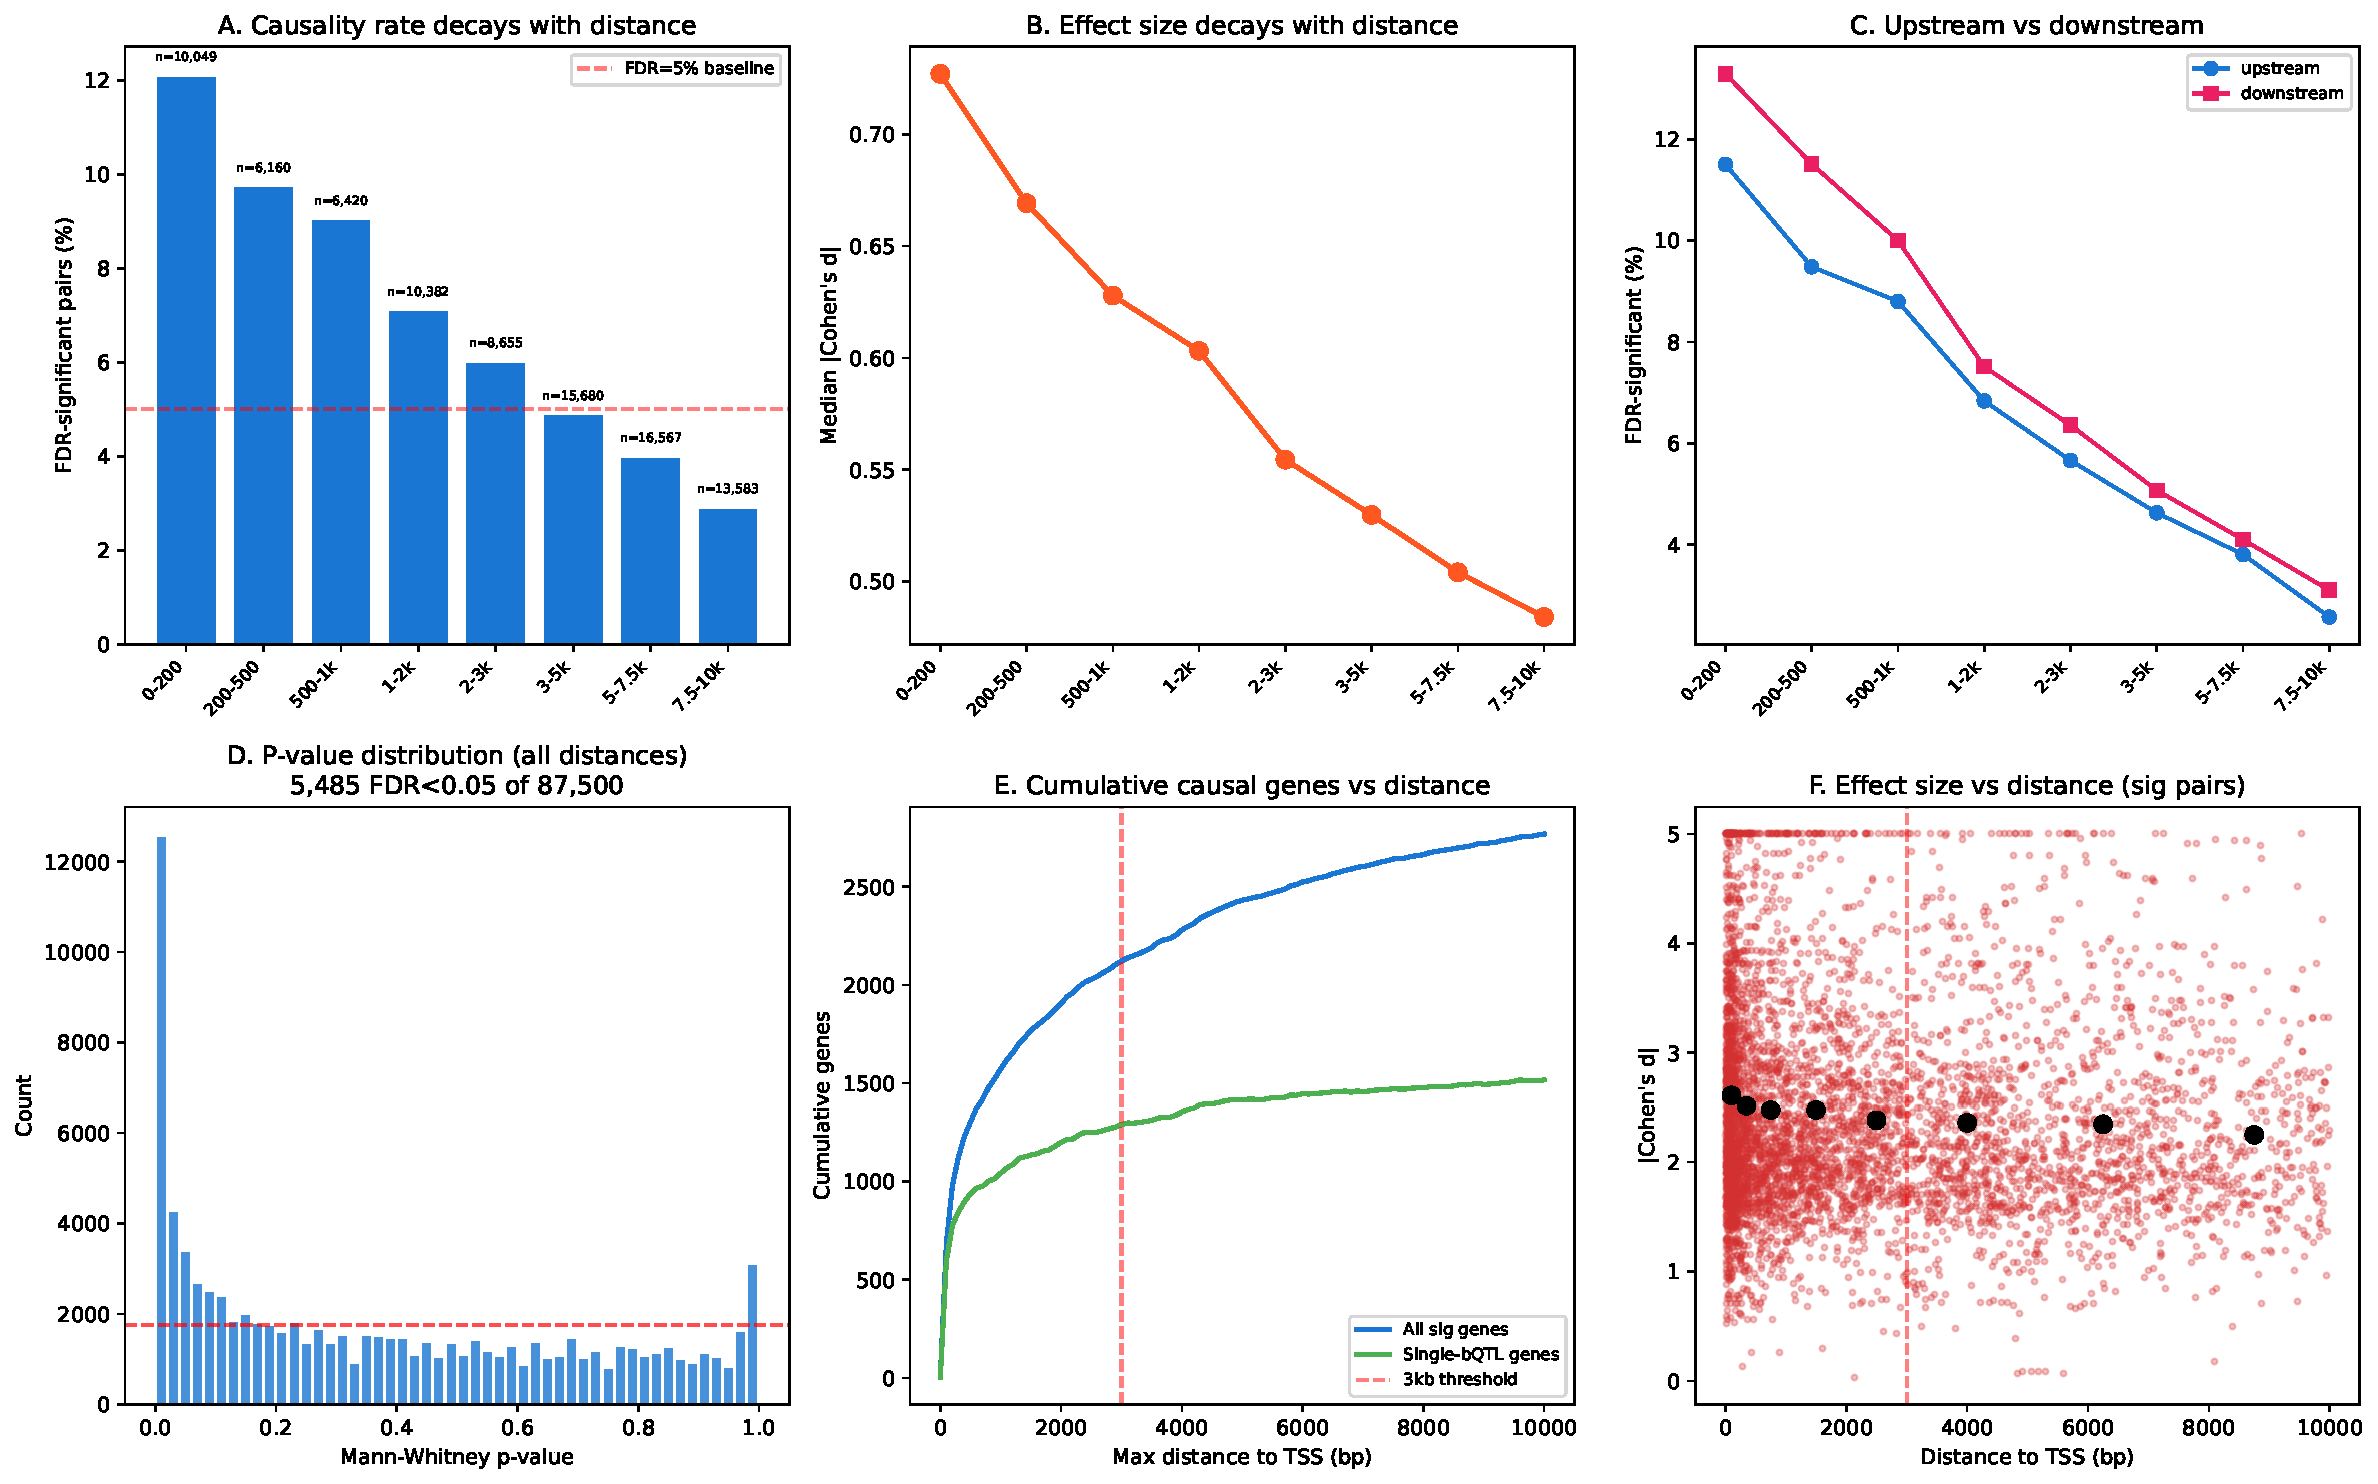
\includegraphics[width=0.7\textwidth]{distance_decay_curve.pdf}
\caption{\textbf{Distance decay of causality rate.}
The fraction of bQTL passing the causal test (FDR\,$<$\,0.05) as a function
of distance from the target gene TSS. The 3\,kb threshold corresponds to
where the rate drops to the 5\% FDR baseline.}
\label{fig:distance_decay}
\end{figure}

\subsection{Motif scanning and redundancy verification}
TF binding motifs were scanned using 405 DAP-seq PWMs (33 TF families) with
a log-odds threshold of 6.0. The variant-overlap constraint required motif
hits to physically overlap the variant nucleotide position ($\pm$28\,bp, the
maximum PWM width). For bidirectional analysis, both the B73 reference and NAM
variant sequences were scanned; motifs present only in the reference were
classified as disrupted, those only in the variant as created.

For sole-copy verification, the tightest MOA-seq binding peak containing each
bQTL was identified across all 25 hybrids, and the number of copies of each
disrupted TF family's motif within that peak was counted. A family was
classified as ``sole copy'' if the variant-overlapping hit was the only
instance within the peak. Multi-family disruption (billboard) analysis tested
the relationship between the number of simultaneously disrupted families and
Cohen's $d$ using Spearman's $\rho$ and linear regression.

Threshold sensitivity was assessed by repeating the bidirectional motif
analysis at seven log-odds thresholds (4.0, 5.0, 5.5, 6.0, 6.5, 7.0, 8.0)
and verifying stability of the zero self-switch finding, motif creation
fractions, and effect size equivalence across categories.

\subsection{Per-hybrid motif linkage}
For each causal bQTL, we reconstructed haplotype-specific binding peak
sequences using founder genotype data and scanned for motif scores across
all 405 PWMs. A motif family was called as a driver if its score significantly
separated variant from reference hybrid groups ($p < 0.05$, Mann--Whitney $U$)
with $\geq$80\% consistency across variants.

\subsection{TF regulatory network}
Directed edges connect disrupting TF families to target genes. Self-loop and
cross-family rewiring rates were tested against null expectations using
binomial tests. Cascade reach was computed as the transitive closure of TF
target sets.

\subsection{Drought pipeline and expression integration}
The causal bQTL pipeline was repeated on drought-stress bQTL (supplementary
Table~S10, 124,504 positions) and ASE data (Table~S13b, 359,162 entries,
23,218 genes, 24 hybrids) using identical parameters. Cross-condition
comparisons used position-level overlap (chr:pos) and gene-level overlap
(gene\_id).

Expression integration cross-referenced causal bQTL targets with
population-level drought expression data (log2FC well-watered vs
drought-stressed) from \citet{engelhorn2025}. Signed allelic effect
correlation with drought direction was tested using Spearman's $\rho$.

\subsection{Functional characterization and comparative enrichment}
Target gene sets were decomposed into WW-only, DS-only, shared-same-variant,
and shared-different-variant groups. Each gene was annotated using EntAP
protein descriptions with keyword-based functional category assignment.
GO enrichment was computed using Fisher's exact test against genome
background, with Benjamini--Hochberg correction. Functional category shifts
between conditions were tested using Fisher's exact test on category
proportions.

\subsection{Population motif occupancy and cross-layer validation}
For each of the 1,126 causal target genes, MOA-seq binding peaks across all
24 hybrids were scanned for TF motif enrichment using 405 DAP-seq PWMs,
building a gene $\times$ TF family $\times$ hybrid occupancy matrix
independent of bQTL identity (Layer~1). TF cascade tracing (Layer~3) followed
directed regulatory chains: bQTL disrupts TF\_A motif $\to$ target gene is
TF\_B $\to$ TF\_B's downstream targets. Conservation-impact scoring combined
motif conservation across hybrids with disruption status to predict ASE
effect magnitude. WW vs DS differential occupancy was tested per TF family
using Wilcoxon signed-rank tests.

\subsection{TF cooperativity}
TF co-occupancy was assessed from the Layer~1 population motif occupancy
matrix. For each TF family pair, co-occurrence at gene promoters was compared
to expectation under independence using Fisher's exact test. Regulatory logic
(additive vs synergistic) was classified based on the relationship between
co-disruption and ASE effect size. Condition-specific cooperativity shifts
were tested by comparing WW and DS co-occupancy matrices.

\subsection{Distributed regulatory architecture}
Per-hybrid causal bQTL burden was computed as the number of causal variants
carried by each hybrid. TF grammar conservation was quantified as pairwise
Spearman correlation of TF family disruption proportions across hybrids.
Gene-level implementation divergence was quantified as pairwise Jaccard
similarity of target gene sets. Functional convergence was assessed by
comparing gene-level Jaccard to GO biological process Jaccard and KEGG
pathway Jaccard. Ancestry-specific modules were identified by hierarchical
clustering of the hybrid $\times$ gene sharing matrix.

\subsection{Hybrid phenotype similarity}
Phenotype data (days to anthesis, plant height, ear height ratio) from
\citet{engelhorn2025} were used to compute pairwise phenotype distance
matrices. Correlation between gene sharing distance and phenotype distance
was tested using the Mantel test with 10,000 permutations.

\subsection{Network topology}
Causal and non-causal target genes were compared for network position metrics
(degree, regulatory entropy, hub status, pairwise Jaccard similarity of
regulatory neighborhoods) within the TF regulatory network. Hub enrichment
was tested using Fisher's exact test.

\subsection{Population genetics}
Allele frequencies were computed from the 24-hybrid genotype matrix. MAF
distributions were compared using the Kolmogorov--Smirnov test.
Effect--frequency correlations used Spearman's $\rho$.

\subsection{Epistasis testing}
For genes with $\geq$2 bQTL, we fitted linear and saturating models to the
relationship between variant allele count and $|$ASE$|$. Model comparison
used AIC, with genes classified as additive (linear AIC $<$ saturating AIC)
or saturating.

\subsection{TE context}
bQTL were intersected with EDTA transposable element annotations
(B73\_NAM5\_TE.gff3.gz, 1.6M elements) using 1\,bp overlap. Enrichment
tested using Fisher's exact test.

\subsection{Chromatin context}
Gene-relative positions were classified as proximal promoter ($\leq$1\,kb),
proximal regulatory (1--3\,kb), or genic (within gene body). Enrichment
versus non-causal bQTL tested using Fisher's exact test.

\subsection{GWAS overlap}
Published GWAS hits from the NGDC GWAS Atlas (42,778 hits, 321 traits, B73v4
coordinates) were intersected with causal bQTL at 100\,kb windows. Trait
enrichment tested using Fisher's exact test with Benjamini--Hochberg
correction.

\subsection{Binding-expression causal chain}
ASE concordance was defined as the fraction of causal bQTL where the variant
allele produces higher $|$ASE$|$ than the reference allele. Dose-response
tested by binning bQTL into effect size quartiles and comparing median ASE.

\subsection{Interactive atlas}
The Maize Causal bQTL Atlas is an interactive HTML visualization built with
D3.js~v7, featuring a force-directed layered cell diagram of all 1,126 genes,
filterable by motif rewiring category, regulatory layer, TF family, drought
response, and specific hybrid.


% ============================================================
\section{Data Availability}
% ============================================================

All bQTL data are from \citet{engelhorn2025}: SRA accession PRJNA1101486,
GEO accession GSE294039. The 1,126-gene atlas, interactive visualization,
and analysis scripts are available at
\url{https://github.com/mbanf/causal-bqtl-atlas}.


% ============================================================
% REFERENCES
% ============================================================

\bibliographystyle{unsrtnat}
\begin{thebibliography}{99}

\bibitem[Engelhorn et al.(2025)]{engelhorn2025}
Engelhorn, J., Snodgrass, S.J., Banf, M., et al. (2025).
A maize leaf pan-cistrome catalogs the cis-regulatory variation underlying
functional trait heritability.
\emph{Nature Genetics}, s41588-025-02246-7.

\bibitem[Boyle et al.(2017)]{boyle2017}
Boyle, E.A., Li, Y.I., Pritchard, J.K. (2017).
An expanded view of complex traits: from polygenic to omnigenic.
\emph{Cell}, 169(7), 1177--1186.

\bibitem[Arnosti and Kulkarni(2003)]{arnosti2003}
Arnosti, D.N. and Kulkarni, M.M. (2003).
Transcriptional enhancers: intelligent enhanceosomes or flexible billboards?
\emph{Journal of Cellular Biochemistry}, 94(5), 890--898.

\bibitem[Finucane et al.(2015)]{finucane2015}
Finucane, H.K., et al. (2015).
Partitioning heritability by functional annotation using genome-wide
association summary statistics.
\emph{Nature Genetics}, 47(11), 1228--1235.

\bibitem[Rutherford and Lindquist(1998)]{rutherford1998}
Rutherford, S.L. and Lindquist, S. (1998).
Hsp90 as a capacitor for morphological evolution.
\emph{Nature}, 396(6709), 336--342.

\bibitem[Marand et al.(2021)]{marand2021}
Marand, A.P., Chen, Z., Gallavotti, A., Schmitz, R.J. (2021).
A cis-regulatory atlas in maize at single-cell resolution.
\emph{Cell}, 184(11), 3041--3055.

\bibitem[Wallace et al.(2014)]{wallace2014}
Wallace, J.G., et al. (2014).
Association mapping across numerous traits reveals patterns of functional
variation in maize.
\emph{PLoS Genetics}, 10(12), e1004845.

\end{thebibliography}


\end{document}
